\documentclass[]{article}
\usepackage{amsmath}
\usepackage{amsfonts}
\usepackage{amssymb}
\usepackage{graphicx}
%opening
\title{Actor Critic Agent}
\author{Marco Marini}

\begin{document}

\maketitle

\begin{abstract}
Description of Actor Critic Agent and definitions of performance indicators
\end{abstract}

\tableofcontents

\section{Actor Critic Agent}

The Policy Actor Critic Agent is composed by an artificial neural network (ANN) that generates the differential state value of critic component and the policy parameters for action selection of each actor (the action space dimensions) from the state input signals.
At each iteration with the environment, the agent computes the average reward $r_\pi$ and the differential TD error $ \delta_t $
\begin{equation}
\delta_t = R_{t+1} - \bar R + \hat v(S_{t+1}) - \hat v(S_t)	
\end{equation}

The differential TD error indicate how different is the differential state value determined by the current reward from the estimated differential state value.

If the error is positive the agent changes the policy reinforcing the current strategy. It increments the probabilities of selected actions and at the same time reduces the probabilities of the other actions.

If the error is negative the agent changes the policy weakening the current strategy. It reduces the probabilities of selected actions and increments the probabilities of the other actions.

The magnitude of changes is proportional to the TD Error by a $ \alpha_i $ parameter for each $ i $ actor that allows to control the convergence of the algorithm.

The TD error is used to determine the updated output values and train the AAN with these expected outputs.

\subsection{Discrete Policy Actor}

The policy actor computes the probabilities $ \pi(a|s) $ of choose action $ a $ at status $ s $.
The probabilities are the softmax function of the action preferences $ h(s,a,\vec \theta) $ given by the ANN 
\begin{align}
	\pi(a|s, \vec \theta)
	&= \frac{e^{h_a(s,a,\vec{\theta})}}{\sum_{b \in A} e^{h(s,b,\vec{\theta})}}
\end{align}

To train the ANN the agent updates the $ \vec \theta $ parameters at each step $ t $
\begin{align}
	\vec \theta_{t+1} =
	\vec \theta_t + \alpha \delta_t \nabla \ln \pi(A_t|S_t, \vec \theta_t) 
\end{align}

The policy gradient function is
\begin{align*}
\begin{split}
	\nabla \ln \pi(A_t|S_t, \vec \theta)
	& = \frac{1}{\pi(A_t|S_t, \vec \theta)}
	\nabla \pi(A_t|S_t, \vec \theta)
	\\
	\pi(a|s, \vec \theta)
	&= \frac{e^{h_a(s,a,\vec{\theta})}}{D(s,\vec \theta)}
	\\
	D(s,\vec \theta)
	&= \sum_{b \in A} e^{h(s,b,\vec{\theta})}
	\\
	\nabla \pi(A_t|S_t, \vec \theta)
	& =
	\frac{1}{D^2(S_t,\vec \theta)}
	\left[
		D(S_t, \vec \theta) \nabla e^{h(S_t,A_t,\vec \theta)} - e^{h(S_t,A_t,\vec \theta)} \nabla D(S_t, \vec \theta)
	\right] 
	\\
	& =	\frac{1}{D^2(S_t,\vec \theta)}
	\left[
		D(S_t, \vec \theta) e^{h(S_t,A_t,\vec \theta)} \nabla h(S_t,A_t,\vec \theta)
		- e^{h(S_t,A_t,\vec \theta)} \nabla D(S_t, \vec \theta)
	\right] 
	\\
	& =
	\frac{\pi(A_t|S_t,\vec \theta)}{D(S_t,\vec \theta)}
	\left[
		D(S_t, \vec \theta) \nabla h(S_t,A_t,\vec \theta)
		- \nabla D(S_t, \vec \theta)
	\right] 
	\\
	\nabla D(s,\vec \theta)
	&= \sum_{b \in A} \nabla e^{h(s,b,\vec \theta)}
	\\
	&= \sum_{b \in A} e^{h(s,b,\vec \theta)}	\nabla h(s,b,\vec \theta)
	\\
	\nabla \pi(A_t|S_t, \vec \theta)
	& =
	\frac{\pi(A_t|S_t,\vec \theta)}{D(S_t,\vec \theta)}
	\left[
		D(S_t, \vec \theta) \nabla h(S_t,A_t,\vec \theta)
		- \sum_{b \in A} e^{h(s,b,\vec \theta)}	\nabla h(s,b,\vec \theta)
	\right] 
\end{split}
\end{align*}

Let be
\begin{align*}
	I(a, b) = 1, \Rightarrow a = b
	\\
	I(a,b) = 0 \Rightarrow a \ne b
\end{align*}
then
\begin{align*}
\begin{split}
	\sum_{b \in A} I(At, b) \nabla h(St, b), \vec \theta)
	&= \nabla h(St, At), \vec \theta)
	\\
	\nabla \pi(A_t|S_t, \vec \theta)
	&=
	\frac{\pi(A_t|S_t,\vec \theta)}{D(S_t,\vec \theta)}
	\sum_{b \in A}
	\left[
		D(S_t, \vec \theta) I(A_t,b)
		-  e^{h(S_t,b,\vec \theta)}
	\right] 	
	\nabla h(S_t,b,\vec \theta)
	\\
	\nabla \ln \pi(A_t|S_t, \vec \theta)
	&=
	\sum_{b \in A}
	\left[
		I(A_t,b)
		-  \pi(S_t,b,\vec \theta)
	\right] 	
	\nabla h(S_t,b,\vec \theta)
	\\
	\delta_h(S_t, A_t, b, \theta_t)
	&= \delta_t
	\left[
		I(A_t,b) - \pi(S_t,b,\vec \theta)
	\right] 
	\\
	\vec \theta_{t+1}
	&=
	\vec \theta_t +
	\sum_{b \in A}
	\alpha \delta_h(S_t, A_t, b, \theta_t)  \nabla h(S_t,b,\vec \theta_t)
\end{split}
\end{align*}

The same result is obtained by training the network with labels
\begin{align}
\begin{split}
	h^*(S_t,A_t,b) = h(S_t,b,\vec \theta_t) + 
	\alpha \delta_h(S_t, A_t, b, \vec \theta_t)
\end{split}
\end{align}

\subsection{Gaussian policy actor}

The Gaussian policy actor computes the probabilities $ \pi(a|s) $ of choose a continuous action $ a $ at status $ s $ as a normal distributed function of two parameters $ \mu(s, \vec \theta_\mu) $ and $ \sigma(s,\vec \theta_h) $.

\begin{align}
	\pi(a|s,\vec \theta_\mu, \vec \theta_h)
	&= \frac{1}{\sigma(s,\vec \theta_h) \sqrt{2 \pi}} e^{-\frac{(a - \mu(s, \vec \theta_\mu))^2}{\sigma(s, \vec \theta_h)^2}}
	\\
	\sigma(s, \vec \theta_h)
	&	= e^{h(s, \vec \theta_h)}	
\end{align}

To train the ANN the agent updates the $ \vec \theta_\mu, \vec \theta_h $ parameters at each step $ t $
\begin{align}
	\vec \theta_{\mu t+1}
	&= \vec \theta_{\mu t}
	+ \alpha_\mu \delta_t \nabla \ln \pi(A_t|S_t, \vec \theta_{\mu t}, \vec \theta_{h t})
	\\
	\vec \theta_{h+1}
	&= \vec \theta_{h t}
	+ \alpha_h \delta_t \nabla \ln \pi(A_t|S_t, \vec \theta_{\mu t}, \vec \theta_{h t})
\end{align}

The policy gradient functions for $\vec \theta_\mu $ is
\begin{align*}
	\nabla \ln \pi(a|s,\vec \theta_\mu, \vec \theta_h)
	& = \pi^{-1}(a|s,\vec \theta_\mu, \vec \theta_h) \nabla \pi(a|s,\vec \theta_\mu, \vec \theta_h)
	\\
	& = \pi^{-1}(a|s,\vec \theta_\mu, \vec \theta_h) \frac{\partial \pi(a|s,\vec \theta_\mu, \vec \theta_h)}{\partial \mu(s, \vec \theta_\mu)} \nabla \mu(s, \vec \theta_\mu)
	\\
	\frac{\partial \pi(a|s,\vec \theta_\mu, \vec \theta_h)}{\partial \mu(s, \vec \theta_\mu)}
	& = - \frac{1}{\sigma^3(s, \vec \theta_h) \sqrt{2 \pi} } e^{-\frac{(a-\mu(s, \vec \theta_\mu))^2}{\sigma^2(s, \vec \theta_h)}} \frac{\partial }{\partial \mu(s,\vec \theta_\mu)} (a-\mu(s, \vec \theta_\mu))^2
	\\
	& = -\pi(a|s,\vec \theta_\mu, \vec \theta_h)  (-2) (a - \mu(s, \vec \theta_\mu)) \sigma^{-2}(s, \vec \theta_h)
	\\
	\nabla \ln \pi(a|s,\vec \theta_\mu, \vec \theta_h)
	& = \frac{2 [a - \mu(s, \vec \theta_\mu)]}{\sigma^2(s, \vec \theta_h)} \nabla \mu(s, \vec \theta_\mu)
\end{align*}
The policy gradient functions for $\vec \theta_h $ is
\begin{align*}
	\nabla \ln \pi(a|s,\vec \theta_\mu, \vec \theta_h )
	& = \pi^{-1}(a|s,\vec \theta_\mu, \vec \theta_h ) \nabla \pi(a|s,\vec \theta_\mu, \vec \theta_h)
	\\
	& = \pi^{-1}(a|s,\vec \theta_\mu, \vec \theta_h )
	\frac{\partial \pi(a|s,\vec \theta_\mu, \vec \theta_h )}{\partial h(s, \vec \theta_h)} \nabla h(s, \vec \theta_h)
	\\	
	\frac{\partial \pi(a|s,\vec \theta_\mu, \vec \theta_h )}{\partial h(s, \vec \theta_h)}
	&= \frac{\partial \pi(a|s,\vec \theta_\mu, \vec \theta_h )}{\partial \sigma(s, \vec \theta_h)}
 	\frac{\partial \sigma(s, \vec \theta_h)}{\partial h(s, \vec \theta_h)}
	\\
	\frac{\partial \pi(a|s,\vec \theta_\mu, \vec \theta_h )}{\partial \sigma(s, \vec \theta_h)}
	& = \frac{
	\left\{
		\sigma(s,\vec \theta_h) \frac{\partial}{\partial \sigma(s,\vec \theta_h)}
		\left[
			e^{-\frac{(a-\mu(s, \vec \theta_\mu))^2}{\sigma^2(s,\vec \theta_h)}}
		\right]
		- e^{-\frac{(a-\mu(s, \vec \theta_\mu))^2}{\sigma^2(s, \vec \theta_h)}}
	\right\}}{\sigma^2(s,\vec \theta_h) \sqrt{2 \pi}}	
	\\
	& = \frac{
	e^{-\frac{(a-\mu(s, \vec \theta_\mu))^2}{\sigma^2(s,\vec \theta_h)}}
	\left\{
		-\sigma(s,\vec \theta_h)
		(a-\mu(s,\vec \theta_\mu))^2
		\frac{\partial}{\partial \sigma(s,\vec \theta_h)}
		\left[
			\sigma^{-2}(s,\vec \theta_h)
		\right]
		- 1
	\right\} }{\sigma^2(s,\vec \theta_h) \sqrt{2 \pi}}	
	\\
	& = \frac{\pi(a|s,\vec \theta_\mu, \vec \theta_h)}{\sigma(s,\vec \theta_h)}
	\left\{
		2 \frac{(a-\mu(s,\vec \theta_\mu))^2} {\sigma^2(s,\vec \theta_h)} - 1
	\right\}
	\\
	\frac{\partial \sigma(s,\vec \theta_h)}{\partial h(s,\vec \theta_h)}
	&= e^{h(s, \vec \theta_h)}
	\\
	&= \sigma(s, \vec \theta_h)
	\\
	\nabla \ln \pi(a|s,\vec \theta_\mu, \vec \theta_h )
	& = 2 \frac{(a-\mu(s,\vec \theta_\mu))^2} {\sigma^2(s,\vec \theta_h)} - 1
\end{align*}

Let be
\begin{align*}
	\delta_\mu(s, a, \vec \theta_\mu, \vec \theta_h )
	&= \delta_t 2 \frac{a - \mu(s, \vec \theta_\mu)}{\sigma^2(s, \vec \theta_h)}
	\\
	\delta_h(s, a, \vec \theta_\mu, \vec \theta_h )
	&= \delta_t 
	\left[
		2 \frac{(a-\mu(s,\vec \theta_\mu))^2} {\sigma^2(s,\vec \theta_h)} - 1
	\right]
\end{align*}

The $ \vec \theta_\mu, \vec \theta_h $ parameters are updated by
\begin{align*}
	\vec \theta_{\mu t+1}
	&= \vec \theta_{\mu t} + \alpha_\mu \delta_\mu(S_t, A_t, \vec \theta_{\mu t}, \vec \theta_{h t} ) 
	\\
	\vec \theta_{h t+1}
	&= \vec \theta_{h t} + \alpha_h \delta_h(S_t, A_t, \vec \theta_{\mu t}, \vec \theta_{ht} ) 
\end{align*}

The same result is obtained by training the network with labels
\begin{align}
	\mu^*(S_t) = \mu(S_t,\vec \theta_{\mu t}) + 
	\alpha_\mu \delta_\mu(S_t, A_t, \vec \theta_{\mu t}, \vec \theta_{ht})
	\\
	h^*(S_t) = h(S_t,\vec \theta_{\mu t}) + 
\alpha_h \delta_h(S_t, A_t, \vec \theta_{\mu t}, \vec \theta_{ht})
\end{align}

\subsection{Learning process}

Initially the agent do not have any experience and the differential state value generated by the ANN starts from a random initial estimation. The same is for the behavior generated by the actors where the preferences are random initialized.

Since the very first interactions the agent generates wrong differential state value estimation with high value of TD Error. Consequently the agent easily changes the policy behavior, trying different policies with the exploration of both the policy and state space. It tries to improve the average reward, the value state estimation at the same time selecting better policies.

Different factors influence the learning process.
External agent factors like the number of states, actions and policies not yet explored tent to generate high error rate.
The error increases as the agent experiences new environment states or try new policies, but as the agent faces states already visited it can exploit the past experiences reducing the error and improving the state value estimation and the policy.

Instead the agent internal factor, such as the ANN approximation, generates errors that can be reduced only to a low-bound limit value.

The ANN learning parameters can influence both in the quality of approximated functions and in the  speed of adaptation.

High value of step-size parameter $ \eta $ increases the correction of weights increasing consequently the speed of adaptation, but can easily generate corrective value too big bringing the network to not converging behaviors.
On the other hand small value of step-size parameter weakens the correction of weights decreasing the speed of adaptation.

Also the actor parameters $ \alpha_i $, which modulate the policy changes from the critic, influence the improvement capacity.
High value of $ \alpha_i $ determine strong policy changes even in the face of small errors, making it difficult a fine correction, the other way around very small value of $ \alpha_a $ bring very little variations on policy without improvement.

If the actor parameters that govern the policy have a limited range of values we may choose an $ \alpha_i = \alpha^*_i $ so that the average of corrections is $ \varepsilon_i $ a fraction of the limited range.

For the discrete policy actors we calculate the average of squared preferences variations $ \Delta^2h_{i} $
\begin{align*}
	h^*_{ia}(t) - h_{ia}(t)&=	\Delta h_{ia}(t)
	\\
	&=	\alpha_i \delta_{h_{ia}}(t)
	\\
	\Delta^2h_{i}(t)&=			\frac{1}{m} \sum_a^m \Delta h_{ia}(t)
	\\
	\Delta^2h_{i}&=			\frac{1}{n} \sum_t^n \Delta^2 h_{i}(t)
	\\
	&=			\frac{1}{n}\frac{1}{m}\sum_t^n \sum_a^m \Delta^2 h_{ia}(t)
	\\
	&=	\alpha^2_i\frac{1}{n}\frac{1}{m}\sum_t^n \sum_a^m  \delta^2_{h_{ia}}(t)
	\\
	\Delta^2h_i &=	\varepsilon^2_i
	\\
	\alpha^*_i&=	\frac{\varepsilon_i}{\sqrt{\frac{1}{n} \frac{1}{m}\sum_t^n \sum_a^m \delta^2 h_{ia}(t)}}
\end{align*}
if $ \alpha_i $ is the value used in the session then
\begin{align}
	\alpha^*_i&=	\frac{\varepsilon_i}{\sqrt{\frac{1}{n} \frac{1}{m} \sum_t^n \sum_a^m \Delta^2 h_{ia}(t)}} \alpha_i
\end{align}

For the Gaussian policy actors we calculate the average of squared parameter variations $ \Delta^2\mu_i$ and $ \Delta^2 h_{i\sigma} $
\begin{align*}
	\mu^*_i(t) - \mu_i(t)&=	\Delta \mu_i(t)
	\\
	&=	\alpha_{i\mu} \delta_{i\mu}(t)
	\\
	\Delta^2\mu_{i}&=			\frac{1}{n} \sum_t^n \Delta^2 \mu_i(t)
	\\
	&=	\alpha^2_{i\mu}\frac{1}{n}\sum_t^n  \delta^2_{\mu_{i}}(t)
	\\
	\Delta^2\mu_i &=	\varepsilon^2_{i\mu}
	\\
	\alpha^*_{i\mu}&=	\frac{\varepsilon_{i\mu}}{\sqrt{\frac{1}{n} \sum_t^n \delta^2 \mu_i(t)}}
\end{align*}
if $ \alpha_{i\mu} $ is the value used in the session then
\begin{align}
	\alpha^*_{i\mu}&=	\frac{\varepsilon_{i\mu}}{\sqrt{\frac{1}{n} \sum_t^n  \Delta^2 \mu_i(t)}} \alpha_{i\mu}
\end{align}

\begin{align*}
	h^*_{i\sigma}(t) - h_{i\sigma}(t)&=	\Delta h_{i\sigma}(t)
	\\
	&=	\alpha_{i\sigma} \delta_{ih_\sigma}(t)
	\\
	\Delta^2h_{i\sigma}&=			\frac{1}{n} \sum_t^n \Delta^2 h_{i\sigma}(t)
	\\
	&=	\alpha^2_{i\sigma}\frac{1}{n}\sum_t^n  \delta^2_{ih_\sigma}(t)
	\\
	\Delta^2h_{i\sigma} &=	\varepsilon^2_{i\sigma}
	\\
	\alpha^*_{i\sigma}&=	\frac{\varepsilon_{i\sigma}}{\sqrt{\frac{1}{n} \sum_t^n \delta^2 h_{i\sigma}(t)}}
\end{align*}
if $ \alpha_{i\sigma} $ is the value used in the session then
\begin{align}
	\alpha^*_{i\sigma}&=	\frac{\varepsilon_{i\sigma}}{\sqrt{\frac{1}{n} \sum_t^n  \Delta^2 h_{i\sigma}(t)}} \alpha_{i\sigma}
\end{align}

\subsection{Performance}

The average reward is the main indicators of learning quality, since the agent interacts with the environment the average reward grows up.

Because the process is adaptive the average reward can vary a lot during the interaction with the environment therefore it is necessary to evaluate the trend of the indicator. The logarithmic regression can be used to evaluate the performance
\begin{align}
	r_\pi(t) & = \ln (mt + q)
\end{align}

An increasing trend indicates the agent is selecting better policies and is getting higher and higher rewards.
A decreasing trend indicates the agent is not selecting good policies, this may be caused by low $ \alpha_a $ or $ \eta $ parameters.

Another indicator of performance is the squared TD error, as for the average reward it is necessary to evaluated the trend.
The error has not negative values that should approach zero when the agent select the local best policy. The exponential regression can be used to evaluate the performance
\begin{align}
	\delta^2(t) & = e^{(mt + q)}
\end{align}

A decreasing trend indicates the estimation of value states is getting better.
An increasing trend indicates the estimation of value states is getting worse it may be caused by the ANN which cannot correct the estimation due to $ \eta $ parameter too high.

Both the critic and actors approximate the value function and policy function with neural network.
To monitor the learning activity of ANN we compute the MSE of estimated functions.


The ANN is feed with normalized values label $ O^*_i $ so that the values are in the range $ -1, +1 $ by linear transformation

\begin{align*}
	O_i &= (O_C, O_{Ai})
	\\
	O_C &= m_c \delta_t + q_c
	\\
	O_{Ai} &= m_{ai} \delta_{hi} + q_{ai}
\end{align*}

The MSE of ANN is
\begin{align*}
	J(t)&	= \sum_i [O^*_i(t) - O_i(t)]^2
\end{align*}
and the MSE after the training is
\begin{align*}
	J'(t)&	= \sum_i [O^*_i(t) - O'_i(t)]^2
\end{align*}

The ratio between the total MSE after and before the training activity indicates the quality of such activity.
\begin{align}
\begin{split}
	K(t)&	= \frac{J'(t)}{J(t)}
\end{split}
\end{align}

A ratio $ K(t) \ge 1 $ means the error after training gets worst due a step-size parameter $ \alpha $ too high.
A ratio $ K(t) = 1 $  means no change on error and therefore no improvement. This can be affected by a local minimum reached or a step-size parameter too low with very poor capacity of learning.
A ratio $ K(t) < 1 $ means an improvement of neural network due to correct step-size parameter.
A ratio $ K(t) = 0 $ means a perfect fit of neural network.

We can classify the steps in three class:
\begin{description}

	\item[$ C_0 $]
	The steps that created a bad approximation with an increased of MSE ($ J > \varepsilon \cup K > 1$)

	\item[$ C_1 $]
	The steps that create a trivial approximation with a small reduction of MSE ($ J > \varepsilon \cup K_0 \le K \le 1 $ with $ K_0 = 0.9$ )

	\item[$ C_2 $]
	The remaining steps that have a small MSE or that have reduced significantly the MSE
\end{description}

The ideal distribution should have 

\begin{align}
\begin{split}
	C_0 & = 0
	\\
	C_1 & = 0
	\\
	C_2 & = 1
\end{split}
\end{align}

A step parameter $ \eta $ too high generates over correction increasing $ C_0 $ and reducing $ C_2 $.

An $ \eta $ parameter too small generates under corrections increasing $ C_1 $ and reducing $ C_2 $.

Because it is difficult to determine the effects of step parameter changes on the result MSE, an empirical way to reduce or increment the parameter is applied, for example increasing or reducing by exponential factors ($ \dots $, $ \times 0.01 $, $ \times 0.03 $, $ \times 0.1$, $\times 0.3 $, $ \times 3 $, $ \times 10 $, $ \times 30$, $\times 100 $, $ \dots $).

\begin{figure}[ht]
	\centering
	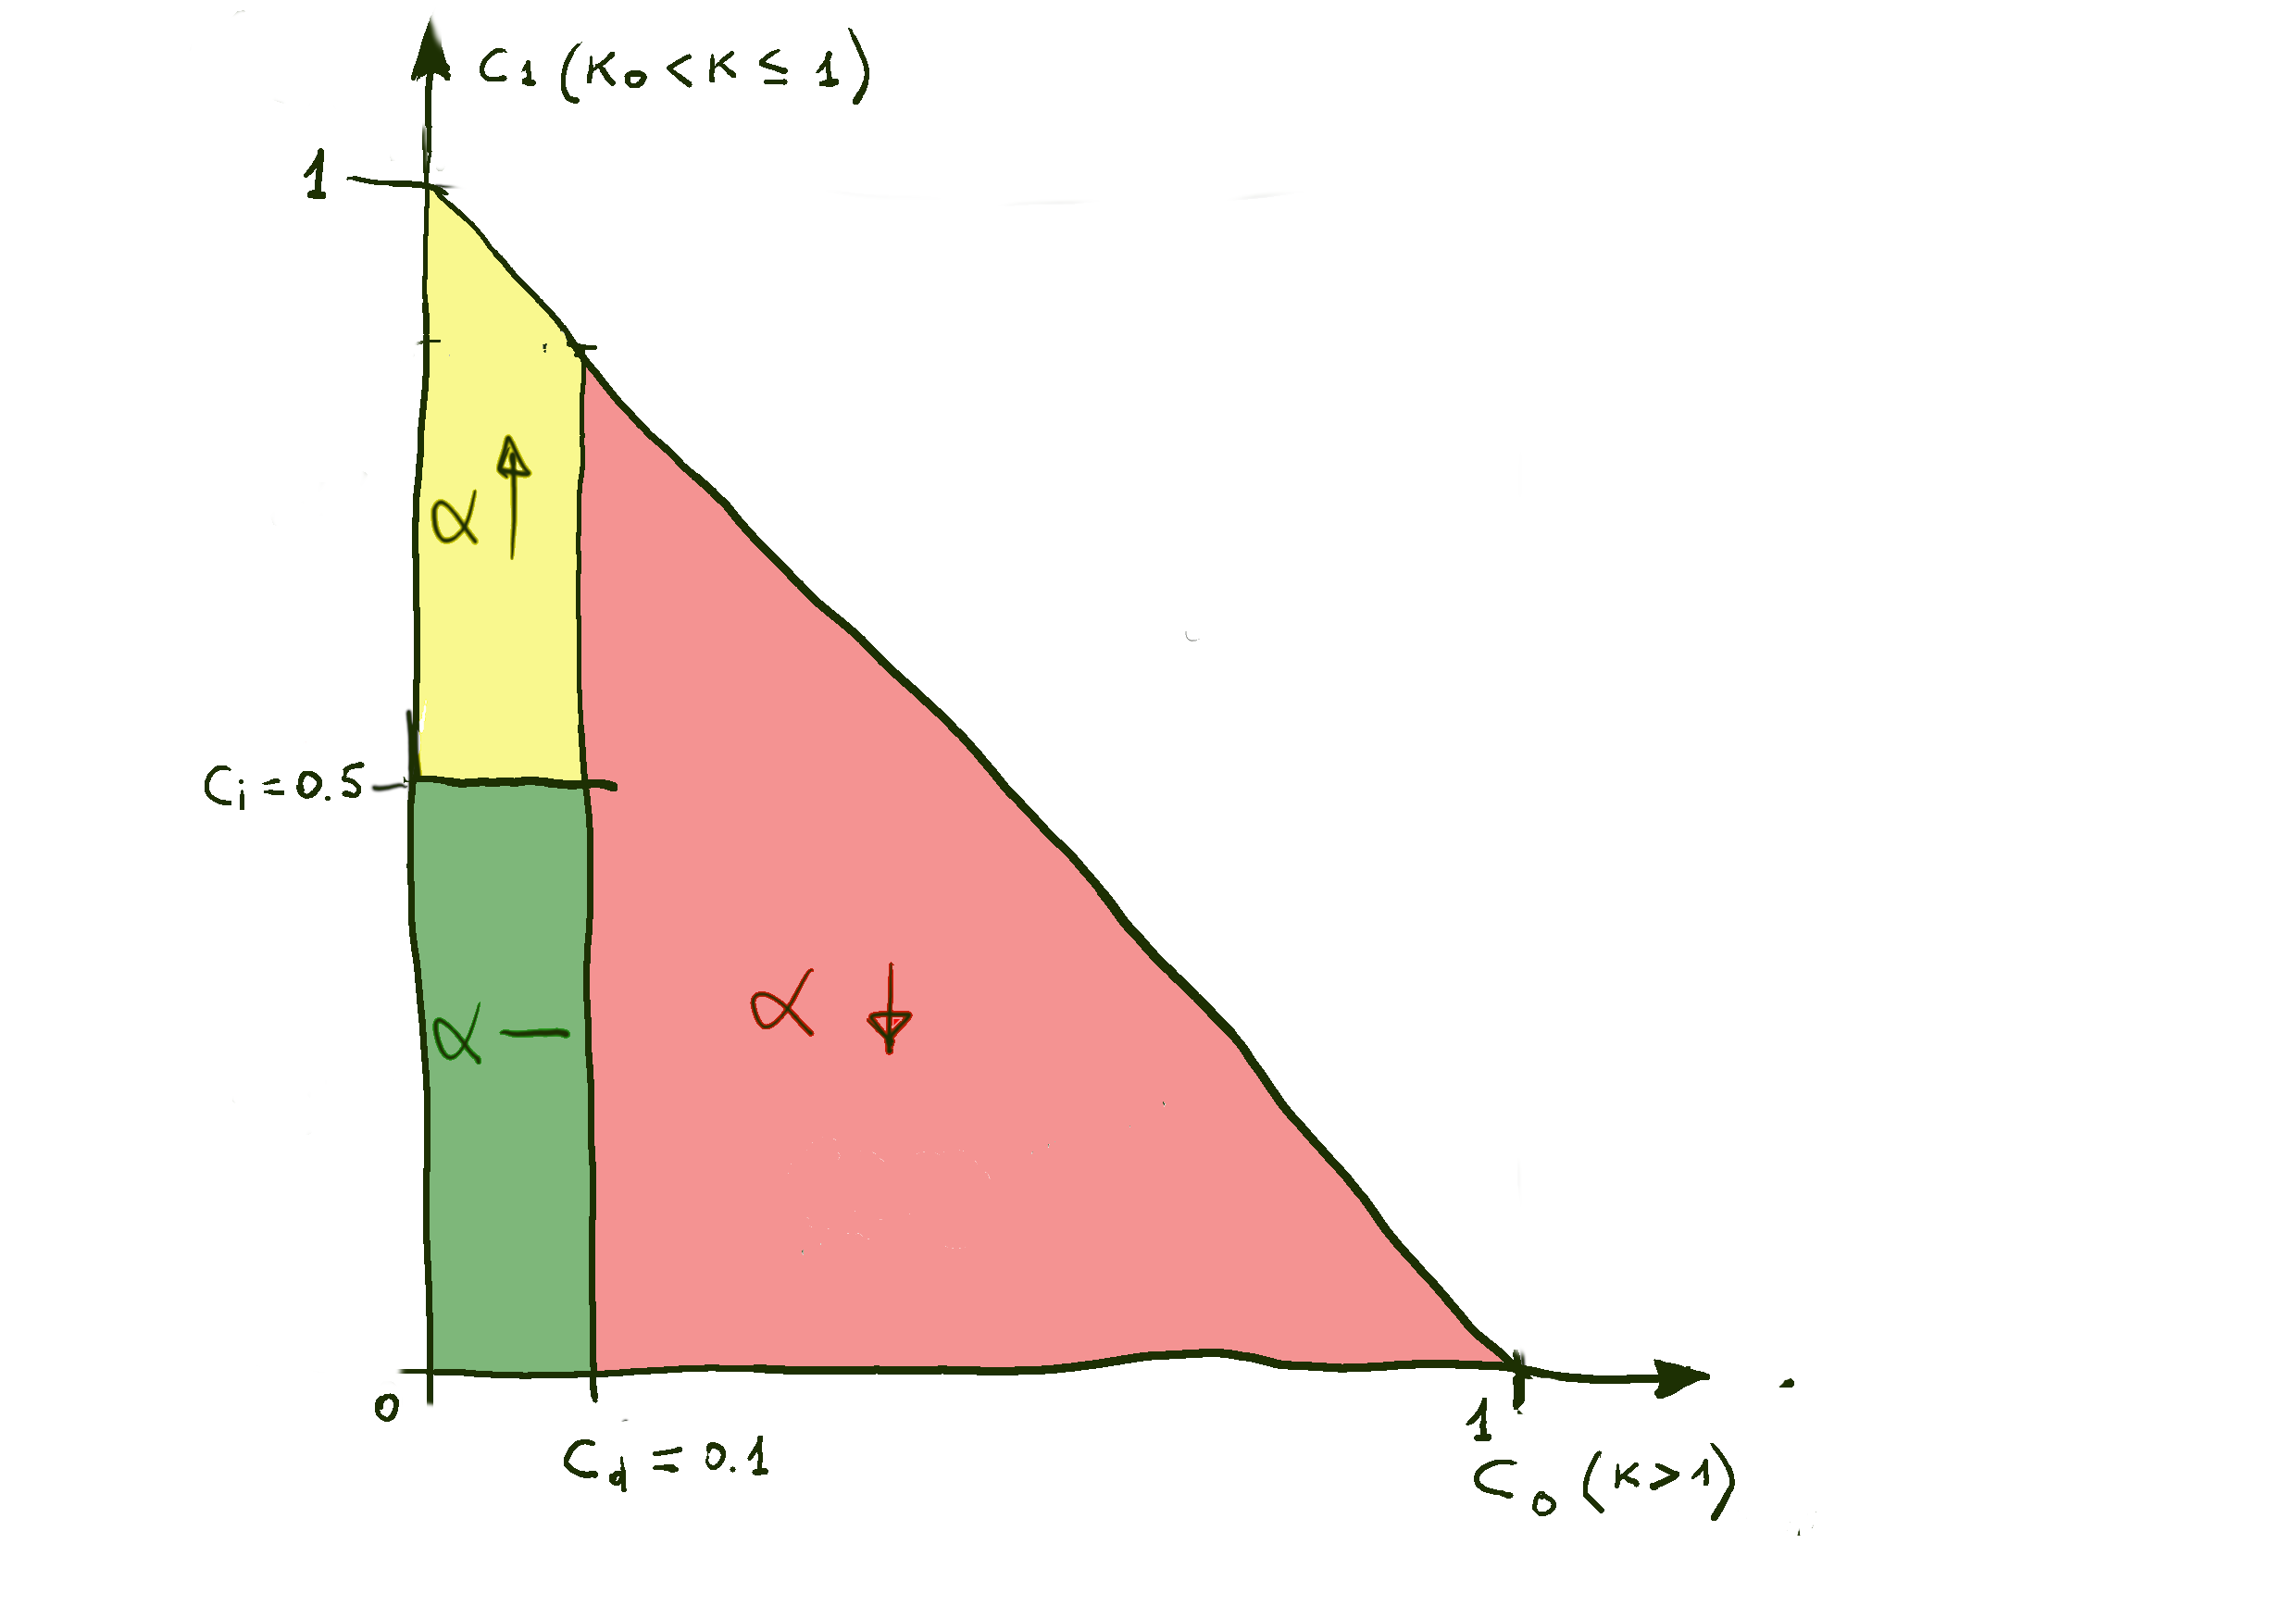
\includegraphics[width=\linewidth]{ann.png}
	\caption{Step classification}
	\label{fig:steps}
\end{figure}

\end{document}
